\section{Introduction}
Le modèle Destinie 2 (modèle Démographique Économique et Social de Trajectoires INdividuelles sImulÉs, version 2) est un modèle de microsimulation dynamique, développé et géré par l’Insee, dont l’objectif principal est la projection à long terme des retraites. Il succède à Destinie 1, premier modèle de microsimulation élaboré sur ce domaine en France, depuis 2010.

\subsection*{Utilisation}
Ce modèle est mobilisé lors des exercices de projection de long terme conduits par le Conseil d’Orientation des Retraites (COR) ou la Commission européenne, mais aussi dans le cadre d'études afin d'éclairer le débat économique et social dans le domaine de la protection sociale (retraites, mais également dépendance ou encore dépenses de santé). En effet, la construction d’un échantillon démographique, couplée à la constitution des liens familiaux et des trajectoires professionnelles, offre au modèle une perspective plus généraliste, qui s’étend au-delà des retraites stricto sensu. Sa dimension « ménages » le distingue d’autres modèles de microsimulation. Par ailleurs, la taille modeste de l'échantillon permet une simulation rapide et ainsi la réalisation de nombreuses variantes, au prix d’une plus faible précision des résultats.


\subsection*{Méthodologie}
Le modèle s’appuie sur un échantillon représentatif de la population française au 1er janvier 2010, construit à partir de l’enquête Patrimoine 2009-2010. Composé d'environ 62 000 individus, cet échantillon initial contient des informations sur les liens familiaux ainsi que l'historique des positions occupées sur le marché du travail. 
La simulation est effectuée au niveau individuel. Le modèle renouvelle la population initiale en simulant des naissances, des décès et des flux migratoires. Il projette ensuite les carrières professionnelles, les revenus d’activité et le départ à la retraite de chaque individu. 
Les personnes en emploi sont réparties en trois grands groupes (les salariés du secteur privé, les titulaires de la fonction publique et les indépendants), comme les retraités (en autant de régimes de base). Ce modèle simplifie un certain nombre d’éléments législatifs (par exemple, les indépendants sont simulés en étant tous soumis aux mêmes règles de calcul des droits). Destinie 2 permet de reconstituer l’ensemble de la trajectoire professionnelle d’un individu (statuts d’activité et revenus) et simule la liquidation de la retraite selon les règles en vigueur pour chaque régime. 

\subsection*{Trois modules principaux}
Le modèle comprend trois modules distincts, écrits en C++ et transcrits en R : le module générateur des biographies démographiques, le module générateur des trajectoires professionnelles et le module «  retraite ».
La construction des trajectoires démographiques s’appuie sur les projections démographiques de l’Insee publiées en 2016, couvrant le champ France entière sur la période 2013-2070. Le nombre de décès, de naissances et les flux migratoires sont ainsi calés chaque année de la projection. 
Les parcours professionnels des individus sont observés jusqu’en 2009, année de base. À compter de 2010, leurs carrières (statuts d’activité et revenus) sont projetées en respectant des contraintes de calage fondées sur des hypothèses macroéconomiques. Ces hypothèses portent sur les gains de productivité du travail, le taux de chômage, tous deux repris des publications du COR, et le taux d’activité, issu des projections de population active de l’Insee.
Le module « retraite » simule le départ à la retraite et calcule le montant des droits associés. Ces droits incluent les droits directs et la pension de réversion des régimes de base (le régime général de la Sécurité sociale, le Service des Retraites de l’État (SRE), la Caisse nationale de retraites des agents des collectivités locales (CNRACL), la Sécurité Sociale pour les Indépendants (SSI)) et de certains régimes complémentaires (Association pour le régime de retraite complémentaire des salariés (Arrco), Association générale des institutions de retraite complémentaire des cadres (Agirc)). Outre la réversion, la dimension « ménages » permet de simuler l’attribution de l’Allocation de Solidarité aux Personnes Âgées (Aspa).
\subsection*{Plusieurs options de simulation}
Le modèle permet une simulation à la carte via un vaste choix d'options. Certaines options permettent d’évaluer la robustesse des résultats obtenus, d'autres ont été rajoutées à l’occasion d’études spécifiques. Les options incluent :
\begin{itemize}
    \item le scénario démographique de l’Insee utilisé en projection relatif à la mortalité, à la fécondité ou encore au solde migratoire.
    \item la législation à appliquer : soit la dernière législation intégrée, soit une précédente législation.
    \item le type de mortalité : prise en compte ou non d'une mortalité différenciée selon le niveau de diplôme.
\end{itemize}    
Les autres options présentes dans le modèle sont documentées sur le dépôt en ligne.


\section{Vue d'ensemble}

Le programme est un package R écrit en C++. Il peut
être directement utilisé à partir d'une console en R, 
pour effectuer des simulations à partir d'un échantillon et de paramètres importés sous R. En revanche, le code source du package est écrit en C++. 

Structure des répertoires du package :

	\begin{description}
		\item[src] contient les fichiers sources du package écrits en C++
		\item[R] contient les fichiers sources du package écrits en R
		\item[parametres] contient les paramètres démographiques et macroéconomiques utilisés lors de la projection\\
Le sous-répertoire {\tt Projections\_COR\_2018} comprend les 5 scénarios économiques du rapport de juin 2018 du COR (voir la table \ref{tab:hypscCOR}). 
\renewcommand{\arraystretch}{1.8}
\newcolumntype{C}{>{\centering\arraybackslash}X}

\begin{table}[h]
  \centering
  \caption{Scénarios économiques du COR}
    \begin{tabular}{rr}
    \toprule
 Gain de productivité du travail (en \%) & Taux de chômage de long terme (en \%) \\
    \midrule
 1,8     & 4,5 \\
 1,8   & 7 \\
 1,5   & 7 \\
 1,3   & 7 \\
 1     & 7 \\
 1     & 10 \\
    \bottomrule
    \end{tabular}%
  \label{tab:hypscCOR}%
\end{table}%
		\item[data] contient un échantillon test \textbf{non représentatif} de la population mais que l'on peut utiliser pour prendre en main le modèle de microsimulation mais aussi des jeux de paramètres du modèle préchargés sous forme d'environnement.
		\item[data\_ raw] contient les scripts R ayant permis d'obtenir les environnements de paramètres et l'échantillon non représentatif. Ces fichiers peuvent être réutilisés pour construire d'autres jeux d'hypothèses.
		\item[demo] contient le script simulation.R permettant de lancer une première simulation avec le modèle.
		\item[documentation] contient la documentation du package, des conseils pratiques, la liste des documents de travail de l'Insee publiés à partir du modèle Destinie 2 et la liste des contributeurs du modèle.
	\end{description}

Le fichier documentation.R permet de réaliser cette documentation en créant une documentation en latex, plus la documentation du package en ligne.




\subsection{Le package Destinie}


Le programme est principalement structuré autour de cinq classes d'objets et de structures (voir la figure \ref{fig:structGenePack}).\\
\begin{description}
\item[La classe Simulation] contient l'ensemble des paramètres de la simulation ainsi que 
l'échantillon issu du générateur de biographies
utilisé sous la forme d'un tableau d'objets Indiv.
\item[La classe Indiv] contient l'ensemble des informations relatives à un individu donné.
\item[La classe Retraite] contient les variables sur les pensions (de droit direct ou dérivé) 
pour un individu et une année donnés.
\item[La classe DroitsRetr] contient l'ensemble des variables concernant la liquidation des
droits directs.
\item[La classe Legislation] contient l'ensemble des paramètres législatifs pour une date de législation, une année et un individu donnés. 
\item[La structure Macro] contient l'ensemble des paramètres macroéconomiques (PIB, inflation,...) mais aussi des 
paramètres plus spécifiques aux retraites (taux de cotisation, valeur des points dans les complémentaires ou encore montant du minimum vieillesse).
\end{description}

De plus, les fichiers {\tt Demographie.cpp}  et {\tt Destinie.h} contiennent les fonctions que l'on peut directement appeler depuis R,
ainsi que les constantes du modèles.
Le fichier {\tt OutilsBase.h} contient des fonctions utilitaires.\\





\phantom{sdfgsdgf
sdfgsdg}

\medskip 

\begin{landscape}
\begin{figure}
\caption{Structure générale du package}
\label{fig:structGenePack}
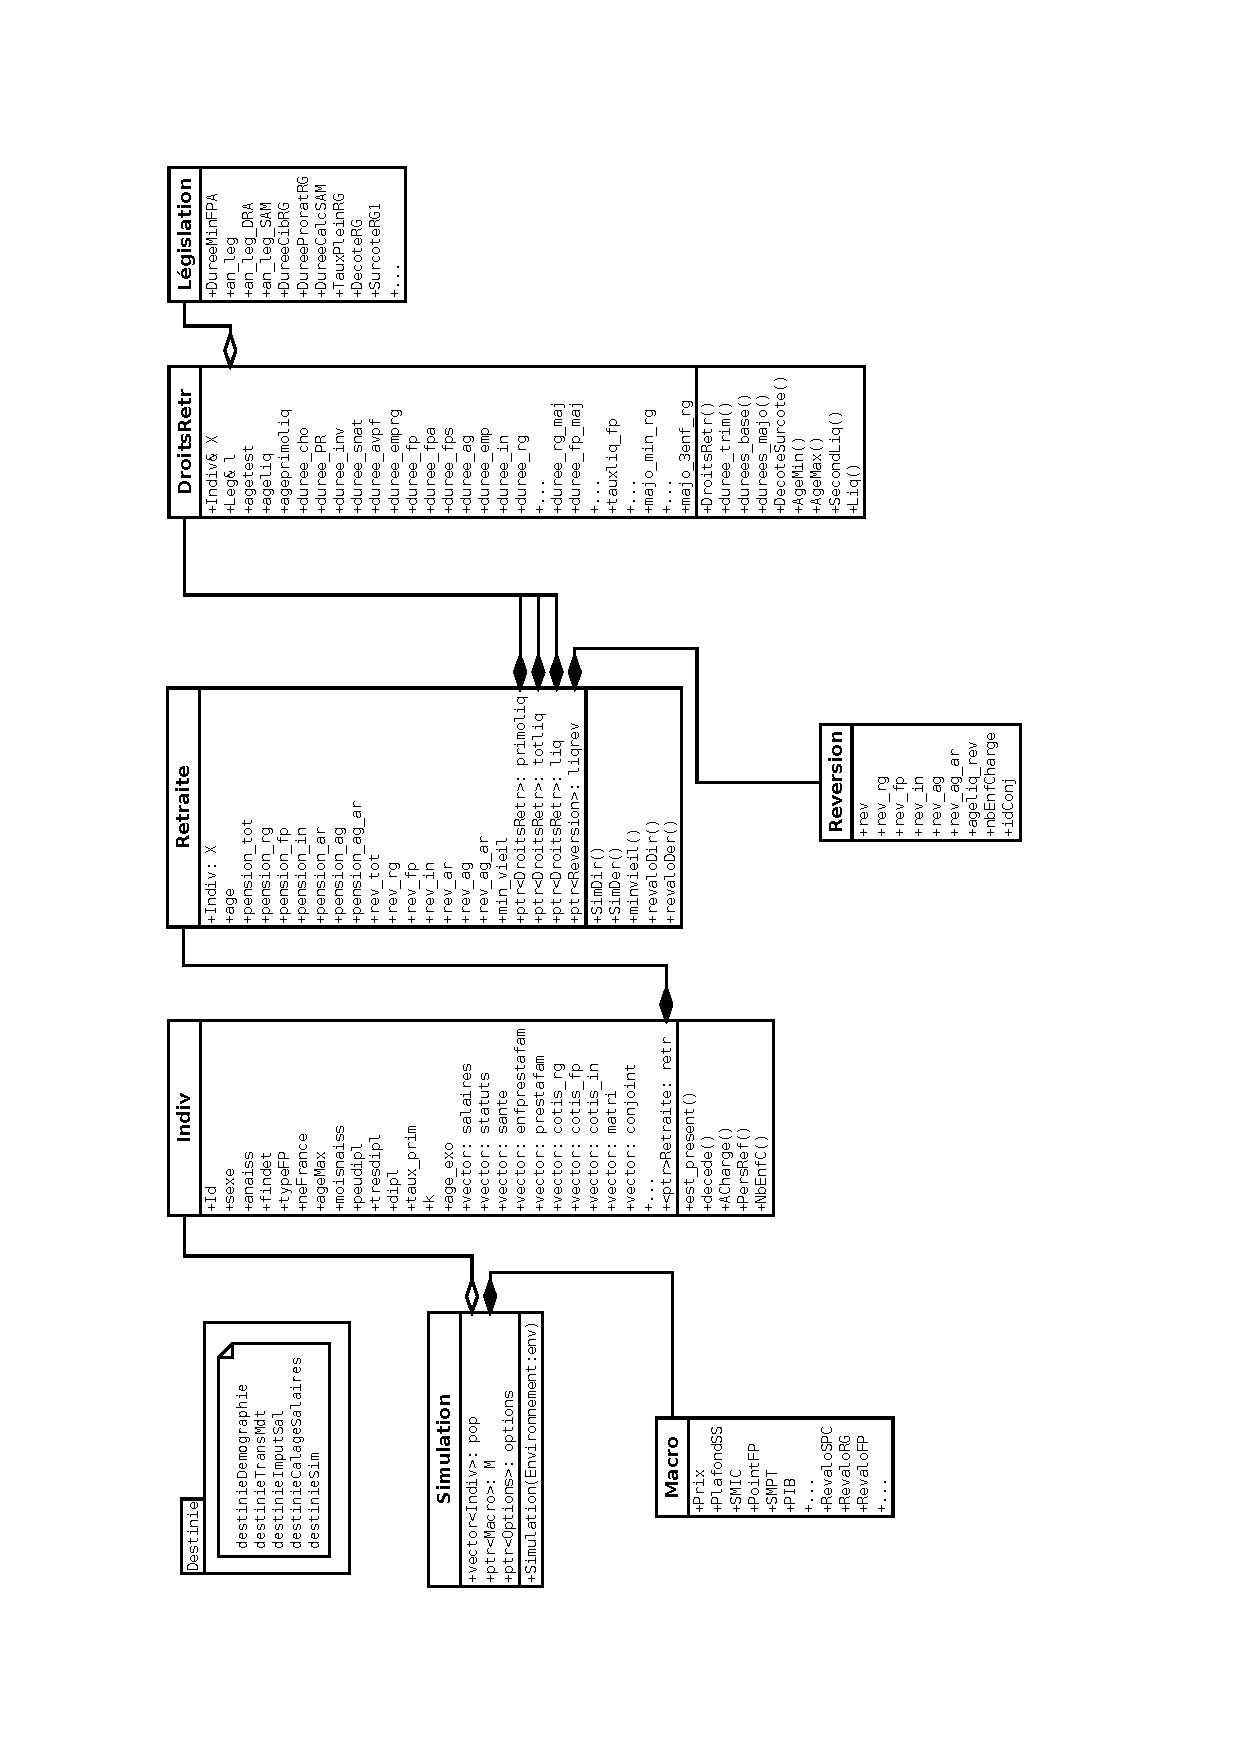
\includegraphics[scale=0.85,angle=270,origin=c]{Diagramme2.pdf}
\end{figure}
\end{landscape}

\subsection{Options et paramètres de simulation}
Un vaste choix d'options et de paramètres permet une simulation à la carte. Ce choix porte sur les hypothèses démographiques, économiques et règlementaires.

\subsubsection{Hypothèses démographiques}
Les scénarios démographiques se distinguent par leurs variantes sur trois composantes que sont la natalité, la mortalité et le solde migratoire. Pour chaque composante, trois variantes existent : centrale (modalité \textit{Cent}), basse (modalité \textit{Bas}), haute (modalité \textit{Haut}). Il existe autant de scénarios que de croisements possibles entre ces variantes, soit 27. Les scénarios s'appuient sur les projections démographiques de l'Insee de 2016, couvrant la période 2013-2070.

\subsubsection{Hypothèses économiques}
Le cadre macroéconomique est défini selon deux axes : le scénario de chômage et de productivité du travail. Trois scénarios de taux de chômage de long terme sont proposés : 4,5 \%, 7 \%, 10 \%. Quant à la productivité, elle évolue selon quatre variantes de croissance tendancielle : 1,0 \%, 1,3 \%, 1,5 \%, 1,8 \%.

\subsubsection{Hypothèses règlementaires et autres}
Avant d'effectuer une simulation, certains paramètres auxiliaires doivent être renseignés dans l'objet \textit{options}. Il s'agit :
\begin{itemize}
\item de la dernière année de législation (variable \textit{anLeg})
\item du mode de comportement de liquidation\footnote{Bien que plusieurs modèles soient proposés, la plupart n'ont pas été expertisés depuis un certain temps. Le choix le plus prudent est celui du départ au taux plein (modalité "tp").}
\item du pas de test de liquidation entre l'âge d'ouverture des droits et l'âge d'annulation de la décote (variable \textit{pas1})
\item du pas de test de liquidation avant l'âge d'ouverture des droits et après l'âge d'annulation de la décote (variable \textit{pas2})
\item de l'horizon de projection (variable \textit{AN\_MAX})
\item du champ de la projection : France entière (modalité "FE") ou métropolitaine (modalité "FM")
\end{itemize}
D'autres options existent et sont détaillées dans la partie \ref{struct_options}. Parmi celles-ci, toutes les options booléennes valent 0 par défaut.

\subsection{Choix de la législation}
La liquidation des droits se fait selon la législation en vigueur à une date choisie par l'utilisateur, stockée dans la variable \textit{anLeg} de l'objet \textit{options}. La législation est alors figée à celle prévalant à cette date.

\subsubsection{Réforme de 1993}

\begin{itemize}
\item	Concerne uniquement les salariés du secteur privé et les régimes alignés ;
\item Allongement progressif de la durée d'assurance requise pour accéder au taux plein (modification progressive pour les générations 1934-1943 à raison d'un trimestre supplémentaire par génération) ;
\item	Calcul du salaire de référence sur les 25 meilleures années au lieu de 10 (modification progressive pour les générations 1934-1947 à raison d'une année supplémentaire par génération) ;
\item	Les pensions et les salaires portés au compte sont indexés sur les prix, et non plus sur les salaires (principe déjà en vigueur depuis 1987) ;
\end{itemize}
\href{http://www.legislation.cnav.fr/textes/cr/cn/TLR-CR_CN_10393_30121993.htm#323}%
{Circulaire n°103/93 du 30 décembre 1993 Caisse nationale d'assurance vieillesse}
% Table generated by Excel2LaTeX from sheet 'Feuil2'
\begin{table}[h]
  \centering
  \caption{Détail par génération de la période transitoire 1993}
    \begin{tabular}{rrr}
    \toprule
    Année de  & Nombre d'années retenues & Trimestres d'assurance  \\
    naissance & pour le calcul du SAM    & pour obtenir le taux plein \\
    \midrule
    1933 et avant & 10    & 150 \\
    1934  & 11    & 151 \\
    1935  & 12    & 152 \\
    1936  & 13    & 153 \\
    1937  & 14    & 154 \\
    1938  & 15    & 155 \\
    1939  & 16    & 156 \\
    1940  & 17    & 157 \\
    1941  & 18    & 158 \\
    1942  & 19    & 159 \\
    1943  & 20    & 160 \\
    1944  & 21    & 160 \\
    1945  & 22    & 160 \\
    1946  & 23    & 160 \\
    1947  & 24    & 160 \\
    1948 et au-delà & 25    & 160 \\
    \bottomrule
    \end{tabular}%
  \label{tab:addlabel}%
\end{table}%


\subsubsection{Réforme de 2003}

\paragraph{Le régime général}

\begin{itemize}
   \item	Allongement progressif de la durée d'assurance requise pour accéder au taux plein à partir de la génération 1949 (passage de 160 
         trimestres à 164)
   \item	Allongement de la durée intervenant dans le coefficient de proratisation, censée à terme évoluer comme la durée cible d'assurance
   \item	Réduction de la décote à partir de la génération 1944, de 0,5 point par an pour atteindre 5\% par annuité manquante pour les 
         générations nées après 1952 (la décote n'est appliquée que si la liquidation a lieu avant 65 ans)
   \item	Surcote de 3 \% par année supplémentaire travaillée après le 1er janvier 2004 ; la surcote a été renforcée par le plan « emploi des 
seniors » au printemps 2005
   \item	Modification du mode de calcul du minimum contributif
   \item	Possibilité de départ anticipé pour carrière longue : depuis le 1er janvier 2004, les assurés qui ont commencé à travailler très 
         jeunes (avant 18 ans), et qui ont eu une longue carrière  peuvent partir à la retraite avant 60 ans (la condition de début de carrière est 
         un obstacle pour les assurés nés à partir de 1953 qui ont connu une scolarité obligatoire jusqu'à 16 ans).
\end{itemize}

% Table generated by Excel2LaTeX from sheet 'Feuil2'
\begin{table}[h]
  \centering
  \caption{Détail par génération de la période transitoire 2003}
    \begin{tabular}{rrrrr}
    \toprule
              &                   & Trimestres    &                       & Trimestres \\
              & Nombre d'années   & d'assurance   & Minoration du taux    & d'assurance   \\
    Année de  & retenues pour     & pour obtenir  & par nombre de         & maximum retenus        \\
    naissance & le calcul du SAM  & le taux plein & trimestre manquant    & pour le calcul RG      \\
    \midrule
    1933 et avant & 10    & 150   & \multicolumn{1}{r}{\multirow{11}[0]{*}{-1,2500}} & \multicolumn{1}{r}{\multirow{11}[0]{*}{150}} \\
    1934  & 11    & 151   & \multicolumn{1}{c}{} & \multicolumn{1}{c}{} \\
    1935  & 12    & 152   & \multicolumn{1}{c}{} & \multicolumn{1}{c}{} \\
    1936  & 13    & 153   & \multicolumn{1}{c}{} & \multicolumn{1}{c}{} \\
    1937  & 14    & 154   & \multicolumn{1}{c}{} & \multicolumn{1}{c}{} \\
    1938  & 15    & 155   & \multicolumn{1}{c}{} & \multicolumn{1}{c}{} \\
    1939  & 16    & 156   & \multicolumn{1}{c}{} & \multicolumn{1}{c}{} \\
    1940  & 17    & 157   & \multicolumn{1}{c}{} & \multicolumn{1}{c}{} \\
    1941  & 18    & 158   & \multicolumn{1}{c}{} & \multicolumn{1}{c}{} \\
    1942  & 19    & 159   & \multicolumn{1}{c}{} & \multicolumn{1}{c}{} \\
    1943  & 20    & \multicolumn{1}{r}{\multirow{6}[0]{*}{160}} & \multicolumn{1}{r}{} & \multicolumn{1}{c}{} \\
    1944  & 21    & \multicolumn{1}{c}{} & -1,1875 & 152 \\
    1945  & 22    & \multicolumn{1}{c}{} & -1,1250 & 154 \\
    1946  & 23    & \multicolumn{1}{c}{} & -1,0625 & 156 \\
    1947  & 24    & \multicolumn{1}{c}{} & -1,0000 & 158 \\
    1948  & \multicolumn{1}{r}{\multirow{5}[0]{*}{25}} & \multicolumn{1}{r}{} & -0,9375 & 160 \\
    1949  & \multicolumn{1}{c}{} & 161   & -0,8750 & 161 \\
    1950  & \multicolumn{1}{c}{} & 162   & -0,8125 & 162 \\
    1951  & \multicolumn{1}{c}{} & 163   & -0,7500 & 163 \\
    1952  & \multicolumn{1}{c}{} & 164   & -0,6875 & 164 \\
    \bottomrule
    \end{tabular}%
  \label{tab:addlabel}%
\end{table}%

\paragraph{Fonction publique}

\begin{itemize}
	\item	Augmentation de la durée d'assurance à partir de 2004 pour rejoindre celle requise dans le régime général et ensuite progresser en 
         parallèle à partir de 2006
	\item	Décote de 0,5 point par annuité manquante, augmentée de 0,5 point à chaque génération pour atteindre 5\% en 2015 (avec hausse 
         progressive de l'âge pivot à partir duquel la décote s'annule)
	\item	Surcote de 3 \% par année supplémentaire travaillée, comme dans le secteur privé
	\item	Modification du mode de calcul du minimum garanti
	\item	Modification des droits familiaux et conjugaux
\end{itemize}



\subsubsection{Réforme de 2010}

\begin{itemize}
	\item  Relèvement progressif de \textbf{l'âge légal de départ} à 
la retraite pour atteindre \textbf{62 ans} en 2018. Cette évolution 
concerne tous les salariés, du public comme du privé ainsi 
que les régimes spéciaux, mais avec des calendriers de mise 
en œuvre différents,
	\item   L'âge à partir duquel il est permis à un assuré, 
n'ayant pas la durée de cotisation requise, de bénéficier 
tout de même d'une retraite à taux plein, passe 
progressivement de \textbf{65 à 67 ans},
	\item   Le dispositif des \textbf{"carrières longues"} est modifié, 
les salariés ayant commencé avant 18 ans peuvent partir à la 
retraite au plus tôt, sous réserve d'avoir la durée de 
cotisation requise pour leur génération, plus 2 ans.
	\item   Pour les salariés qui, du fait d'une situation 
d'usure professionnelle, ont une incapacité physique 
supérieure ou égale à 20 \%, l'âge légal de départ à la 
retraite reste fixé à 60 ans et aucune décote ne leur est 
appliquée. \textit{Dispositif non intégré dans le modèle.}
	\item   Les jeunes en chômage non indemnisé peuvent 
valider jusqu'à 6 trimestres (au lieu de 4).
	 \item    pour les femmes, l'indemnité journalière perçue 
 pendant le congé maternité entrera dans le salaire de 
 référence sur lequel sera calculée la pension de retraite. \textit{Dispositif non intégré dans le modèle.}
	 \item    de nouvelles recettes financières sont instaurées, 
 comme la hausse de la tranche la plus élevée de l'impôt sur 
 le revenu (41 \% au lieu de 40 \%), l'augmentation des 
 taxes sur les stock-options et les retraites-chapeaux, le 
 relèvement des prélèvements forfaitaires sur les revenus du 
 capital et des taxes sur les dividendes perçus par les 
 actionnaires. \textit{Dispositif non intégré dans le modèle.}
	 \item    l'objectif assigné au fonds de réserve des 
 retraites est modifié : ses réserves (36,2 milliards en 2010)
  seront, à partir de 2011, ponctionnées annuellement (2,1 
 milliards) au profit de la Caisse d'amortissement de la 
 dette sociale (Cades). \textit{Dispositif non intégré dans le modèle.}
\end{itemize}

\subsubsection{Accélération du calendrier fixé en 2010 suite au projet de loi de financement de la sécurité sociale pour 2012}
La loi du 21 décembre 2011 relative au financement de la sécurité sociale en 2012 prévoit une accélération de la réforme de 2010 : l'âge légal de départ et l'âge d'annulation de la décote passent à 62 et 67 ans respectivement, dès 2017 au lieu de 2018.

\subsubsection{Décret de juillet 2012: extension du dispositif carrières longues}

Le décret du 2 juillet 2012 étend le dispositif de départs anticipés pour carrière longues, à compter de novembre 2012, aux personnes qui ont commencé à travailler avant 20 ans, et en supprime la condition relative à la durée d'assurance totale (la condition relative à la durée d'assurance cotisée est maintenue mais aménagée).

\subsubsection{Réforme de 2013}
\begin{itemize}
   \item Augmentation de la durée de cotisation d'un trimestre tous les 3 ans à partir de la génération née en 1958 pour atteindre 43 ans pour la génération 1973.
   \item Les périodes d'apprentissage, la formation, le chômage et la maternité sont mieux pris en compte. \textit{Dispositif non intégré dans le modèle.}
   \item Un trimestre est considéré comme validé dès que le salarié a cotisé 200 heures au Smic. Ce seuil passe à 150 heures au bénéfice des personnes à temps très partiel, avec un plafond fixé à 1,5 Smic. \textit{Dispositif non intégré dans le modèle.}
   \item Pour les salariés du public comme du privé, les cotisations patronales et salariales sont augmentées de 0,15 point chacune dès le 1er janvier 2014, puis de 0,05 point en 2015, 2016 et 2017.
   \item Mise en place d'un compte pénibilité. \textit{Dispositif non intégré dans le modèle.}
   \item Le bonus pour les parents de trois enfants est fiscalisé. \textit{Dispositif non intégré dans le modèle.}
   \item La revalorisation des pensions est décalée de six mois chaque année.
   \item Mise en place de la Lura (Liquidation unique des régimes alignés) à compter du 1er juillet 2017. Pour les individus ayant été affiliés à au moins deux des trois régimes alignés (régime général, régime social des indépendants et MSA-salariés), et dont la liquidation intervient à partir du 1er juillet 2017, la pension est calculée de façon unifiée. Le salaire de référence est calculée sur la base des 25 meilleures années (tous régimes confondus), et la durée validée par année est bornée à quatre trimestres (par exemple, pour un individu ayant validé quatre trimestres au régime général et deux trimestres au RSI au cours d'une année, seuls quatre trimestres sont pris en compte dans la durée d'assurance). Le versement de la pension, due au titre des droits ouverts dans les trois régimes alignés, est assuré par le dernier régime d’affiliation. Sur ce point, Destinie 2 s'écarte de la législation : la pension est proratisée en fonction des durées validées dans chaque régime et les proratas sont comptés à la charge des régimes concernés. Cet écart permet d'évaluer les dépenses effectivement engagées par les régimes.
\end{itemize}

\subsubsection{Accord national interprofessionnel relatif aux retraites complémentaires Agirc-Arrco du 30 octobre 2015}
\begin{itemize}
   \item En 2016, 2017 et 2018, indexation de la valeur du service des points Agirc et Arrco sur l'inflation moins un point.
   \item En 2016, 2017 et 2018, indexation de la valeur d'achat des point Agirc et Arrco sur l'évolution du SMPT augmentée de deux points.
   \item Extension de la cotisation AGFF sur la tranche B à la tranche C à compter du 1er janvier 2016.
   \item Pour les individus liquidant leur retraite de base au taux plein, application d'un coefficient de minoration de 10\% sur la pension complémentaire, et ce, pour une durée de trois ans dans la limité de l'âge d'annulation de la décote. Ce coefficient ne s'applique pas aux individus qui liquident un an au moins après avoir rempli les conditions du taux plein. Pour les individus exonérés de la CSG ou soumis à un taux réduit, le coefficient ne s'applique pas ou est réduit.
   \item Pour les individus remplissant les conditions du taux plein dans les régimes de base mais reportant leur liquidation de la retraite complémentaire d'au moins deux années, application, pour une durée d'un an, d'un coefficient majorant :
   \begin{itemize}
   \item de 10 \% si la liquidation a lieu au moins deux ans après
   \item de 20 \% si la liquidation a lieu au moins trois ans après
   \item de 30 \% si la liquidation a lieu au moins quatre ans après
   \end{itemize}
\end{itemize}



